\section{Operators on the super-loop and their eigenvalues}
\label{sec:operators}

\subsection{Derivations and automorphisms}

An \emph{automorphism} of $\mathbb B_{\rm LL}$ is an invertible linear map that preserves the product;
a \emph{derivation} is its infinitesimal form, a linear map $\mathcal D_{\rm LL}$ with
$\mathcal D_{\rm LL}(\mathbf x\mathbf y)=(\mathcal D_{\rm LL}\mathbf x)\mathbf y+\mathbf x(\mathcal
D_{\rm LL}\mathbf y)$. Automorphisms map $\mathbb L_{\rm LL}$ to itself, so they are
symmetries of the super-loop that act on it from outside; they are linear operators on
$\mathbb B_{\rm LL}$ and, unlike the elements of the loop, compose associatively. Two families
matter (L-7):
\begin{align}
D_{\rm LL}(\mathbf u)(\mathbf a+\mathbf b\,\mathbf e_4)&=[\mathbf u,\mathbf a]+(-\mathbf b\mathbf u)\,\mathbf e_4,\label{eq:dlor}\\
D^{\rm v}_{\rm LL}(\mathbf t)(\mathbf a+\mathbf b\,\mathbf e_4)&=(\mathbf t\mathbf b)\,\mathbf e_4,\label{eq:diso}
\end{align}
for a Lorentz element $\mathbf u\in\mathfrak l_{\rm LL}$ and an isospin element $\mathbf t\in{\rm
Im}\,\mathbb H$. Both are derivations (checked on random pairs), they commute with each other, and
the isospin derivations vanish on $\mathbb C\otimes\mathbb H$. Integrated, they give the automorphisms
\begin{equation}
\varphi^{\rm LL}_{\mathbf g,\mathbf v}(\mathbf a+\mathbf b\,\mathbf e_4)=\mathbf g\mathbf a\bar{\mathbf g}+(\mathbf v\mathbf b\bar{\mathbf g})\,\mathbf e_4
\label{eq:aut}
\end{equation}
for unit bi-quaternions $\mathbf g$ (a Lorentz transformation) and $\mathbf v$ (an isospin rotation)
(L-9); together they form $(SL(2,\mathbb C)\times SL(2,\mathbb C))/\mathbb Z_2=SO(4,\mathbb C)$.
All derivations of $\mathbb B_{\rm LL}$ form the complex exceptional Lie algebra $\mathfrak g_2(\mathbb
C)$, of real dimension 28: the linear conditions for a derivation have rank {{GEN:der_rank}} for the 256
entries of a real $16\times16$ matrix, and the inner derivations $[L^{\rm LL}_{\mathbf x},L^{\rm
LL}_{\mathbf y}]+[L^{\rm LL}_{\mathbf x},R^{\rm LL}_{\mathbf y}]+[R^{\rm LL}_{\mathbf x},R^{\rm
LL}_{\mathbf y}]$ (with the right multiplications $R^{\rm LL}_{\mathbf y}$) span {{GEN:der_span}}
dimensions (L-8). The automorphism group is $\mathrm G_2(\mathbb C)$, and $SO(4,\mathbb C)$ is the part
of it that keeps $\mathbb C\otimes\mathbb H$ in place.

\subsection{The operators and their eigenvalues}

The super-loop carries the following operators, all built from Eqs.~(\ref{eq:dlor})
and~(\ref{eq:diso}); their eigenvalues are collected in Fig.~\ref{fig:charges}.

\emph{Isospin and electric charge.} The isospin generators $T^\iota_{\rm LL}=i\,D^{\rm v}_{\rm
LL}(\mathbf e_\iota/2)$ ($\iota=1,2,3$) are Hermitian and obey $[T^1_{\rm LL},T^2_{\rm LL}]=iT^3_{\rm
LL}$ and its cyclic permutations. We call the third one the \emph{electric charge},
$Q_{\rm LL}=T^3_{\rm LL}$. It has the eigenvalue 0 on $\mathbb C\otimes\mathbb H$ (four times) and the
eigenvalues $+\tfrac12$ and $-\tfrac12$ (twice each) on the spinor charges (Q-1); the isospin Casimir
$(T_{\rm LL})^2=\sum_\iota(T^\iota_{\rm LL})^2$ is 0 on $\mathbb C\otimes\mathbb H$ and
$\tfrac34=\tfrac12(\tfrac12+1)$ on the spinor charges, which are therefore an isospin doublet (Q-2).

\emph{Spin.} The Casimir of the rotations, $\mathrm{Cas}_{\rm LL}=-\sum_jD_{\rm LL}(J^j_{\rm LL})^2$, has
the eigenvalue 0 on $\mathbf e_0$ (spin 0), 2 on the Lorentz part (spin 1) and $\tfrac34$ on the
spinor charges (spin $\tfrac12$) (Q-3, exact).

\emph{Chirality.} Because $D_{\rm LL}$ is complex-linear in its argument and $K^j_{\rm LL}=iJ^j_{\rm
LL}$, every boost acts as $i$ times the corresponding rotation on every bi-octonion,
$D_{\rm LL}(K^j_{\rm LL})=i\,D_{\rm LL}(J^j_{\rm LL})$ (Q-4). A Lorentz multiplet on which the rotations
act with spin $\tfrac12$ (or 1) and the boosts as $i$ times the rotations is said to be of type
$(\tfrac12,0)$ (or $(1,0)$); with $-i$ in place of $i$ it is of type $(0,\tfrac12)$ (or $(0,1)$). So the
spinor charges are of type $(\tfrac12,0)$ and the Lorentz part of type $(1,0)$: the super-loop has one
chirality. The complex-conjugate super-loop, in which every coefficient is replaced by its complex
conjugate, has the other.

\emph{Spinor number.} The rotation by the angle $2\pi$ about the third axis, $\exp(2\pi D_{\rm
LL}(J^3_{\rm LL}))$, is $+1$ on $\mathbb C\otimes\mathbb H$ and $-1$ on the spinor charges, because
$iD_{\rm LL}(J^3_{\rm LL})$ has the integer eigenvalues $-1,0,0,1$ on the first and the eigenvalues
$\pm\tfrac12$ on the second (Q-5): the spinor charges are fermionic in their Lorentz quantum numbers,
although they are elements of an algebra with a commutator.

\emph{Twist charge.} $\Theta_{\rm LL}$, Sec.~\ref{sec:superloop}, is 1 on $\mathfrak l_{\rm LL}$ and
$-2$ on $\mathfrak s_{\rm LL}$. It is a new quantity: it measures by how much the inner action of the
Lorentz part fails to be a representation, Eq.~(\ref{eq:jacluu}), and Theorem M will show that $0$, $1$
and $-2$ are the only values that a Malcev algebra allows. Its value $-2$ appears directly in the loop:
conjugation by an element $\mathbf g$ of $SL(2,\mathbb C)$ acts on a spinor charge as
\begin{equation}
\mathbf g(\mathbf b\,\mathbf e_4)\bar{\mathbf g}=(\mathbf b\,\mathbf g^2)\,\mathbf e_4
\label{eq:conj}
\end{equation}
(Q-6; both orders of the two products agree), whereas the automorphism~(\ref{eq:aut}) acts as
$\mathbf b\mapsto\mathbf b\bar{\mathbf g}=\mathbf b\,\mathbf g^{-1}$: the loop's own conjugation turns a
spinor charge twice as fast and in the opposite sense.

\begin{figure}[t]
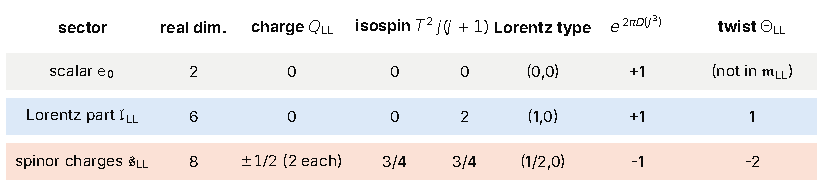
\includegraphics[width=\columnwidth]{../figures/fig_sl_charges.pdf}
\caption{Quantum numbers of the three sectors of $\mathbb B_{\rm LL}$ under the operators of
Sec.~\ref{sec:operators}: the electric charge $Q_{\rm LL}$, the isospin Casimir, the spin Casimir
$\mathrm{Cas}_{\rm LL}$, the Lorentz type, the spinor number $\exp(2\pi D_{\rm LL}(J^3_{\rm LL}))$ and the
twist charge $\Theta_{\rm LL}$ (checks Q-1 to Q-6, L-7).}
\label{fig:charges}
\end{figure}

\subsection{The inversion element}

The unit $\mathbf e_4$ itself is an element of the super-loop with $\mathbf e_4^2=-\mathbf e_0$ and
$\mathbf e_4^{-1}=-\mathbf e_4$. Conjugation by it acts on the bi-quaternions by
\begin{equation}
\mathbf e_4\,\mathbf a\,\mathbf e_4^{-1}=\bar{\mathbf a}
\label{eq:inversion}
\end{equation}
(C-1). On $SL(2,\mathbb C)$ this is the inversion $\mathbf g\mapsto\bar{\mathbf g}=\mathbf g^{-1}$, and on
the Minkowski space $\mathbb R^{1,3}_{\rm LL}$ of the Hermitian bi-quaternions $x^0_{\rm LL}\mathbf
e_0+i\sum_jx^j_{\rm LL}\mathbf e_j$ (Sec.~\ref{sec:manifolds}) it is the parity
$x^j_{\rm LL}\mapsto-x^j_{\rm LL}$. The union of $SL(2,\mathbb C)$ and $SL(2,\mathbb C)\,\mathbf e_4$ is
closed under the product, by Eq.~(\ref{eq:cd}):
\begin{align}
(\mathbf g\,\mathbf e_4)(\mathbf h\,\mathbf e_4)&=-\bar{\mathbf h}\mathbf g,\qquad \mathbf g(\mathbf h\,\mathbf e_4)=(\mathbf h\mathbf g)\,\mathbf e_4,\nonumber\\
(\mathbf g\,\mathbf e_4)\mathbf h&=(\mathbf g\bar{\mathbf h})\,\mathbf e_4
\label{eq:chein}
\end{align}
(C-2). It is a Moufang loop of the type constructed by Chein~\cite{Chein1974}, a ``double'' of the
Lorentz group, and it is not associative because $SL(2,\mathbb C)$ is not commutative.

Such an element cannot exist in a group. In a group, conjugation by an element is an automorphism, and
the inversion $\mathbf g\mapsto\mathbf g^{-1}$ of $SL(2,\mathbb C)$ is not one: for $\mathbf g=\mathbf e_1$
and $\mathbf h=\mathbf e_2$, $(\mathbf g\mathbf h)^{-1}=-\mathbf e_3$ but $\mathbf g^{-1}\mathbf
h^{-1}=+\mathbf e_3$ (C-3). In the loop, conjugation by $\mathbf e_4$ is not an automorphism of
$\mathbb B_{\rm LL}$ (C-4), and the inversion is realized by an element. This is a third way in which
the super-loop goes beyond what H-grp allows.
